\documentclass[11pt,a4paper]{article}
\usepackage[margin=2.1cm]{geometry}
\usepackage{amsmath,booktabs,tabularx,xcolor,hyperref,enumitem,graphicx,float,listings,longtable}
\usepackage{tikz}
\usetikzlibrary{positioning,arrows.meta,fit}
\hypersetup{colorlinks,linkcolor=blue!50!black,urlcolor=blue!50!black}
\setlist{itemsep=1pt,topsep=2pt}
\newcommand{\code}[1]{\texttt{\small #1}}
\definecolor{bad}{HTML}{B5403A}\definecolor{good}{HTML}{2E7D4F}\definecolor{warn}{HTML}{B07A12}
\lstset{language=Python,basicstyle=\ttfamily\footnotesize,columns=fullflexible,keepspaces,
  frame=single,framerule=0.3pt,rulecolor=\color{gray!60},backgroundcolor=\color{gray!4},
  commentstyle=\color{gray!70!black},keywordstyle=\color{blue!50!black},breaklines,showstringspaces=false}
\tikzset{box/.style={draw,rounded corners=2pt,align=center,font=\small,inner sep=4pt,minimum width=2.6cm},
  dom/.style={box,fill=good!10},infra/.style={box,fill=blue!6},orch/.style={box,fill=warn!12},
  dep/.style={-{Stealth[length=2mm]},thick,gray!70!black}}

\title{Credit Risk Workbench: how to build it\\[2pt]\large Ideation, architecture, design and a review of the design}
\author{risk-workbench}
\date{25 October 2026. Source: \code{credit-risk-workbench-design-brief.md} v1.0}

\begin{document}
\maketitle

\noindent\fcolorbox{gray}{gray!6}{\parbox{\dimexpr\linewidth-2\fboxsep-2\fboxrule}{%
\textbf{The answer}
\begin{enumerate}
\item \textbf{The data layer becomes a contract, not a database.} The brief's Section 9 tables become canonical tables. Each table has fixed columns, units, a sign rule and two clocks: \code{effective\_at} (when it was true) and \code{available\_at} (when it was known).
\item \textbf{One narrow port reads them.} A \code{Source} has one method: \code{read(kind, window)}. This machine plugs in a synthetic source and a parquet-tables source. The work machine plugs in its own adapter by setting \code{CRW\_SOURCE=module:factory}. No other code changes.
\item \textbf{Every run freezes what it read.} The run copies its inputs into an archive. The archive is itself a \code{Source}, so any old report replays exactly, even after the work database revises.
\item \textbf{The calculations never touch the data layer.} They are pure functions on canonical tables. Orchestration reads, calls them, and writes results. The screens read results only.
\item \textbf{This machine proves the method on synthetic data.} It has no book and no official P\&L. A synthetic market with known factor moves is the test oracle. The brief's Section 10 checks become the acceptance tests.
\end{enumerate}
\textbf{The review rates the design \color{good}sound\color{black}, with three things to fix before code} (Section~\ref{sec:review}). The most important: the read-recorder must not be shared across parallel workers.

\textbf{Agreed in review (Section~\ref{sec:agreed}, overrides earlier sections):} semi-live runs (start of day, refresh, end of day); CP+ intraday prices with per-bond staleness; FINCAD analytics behind a new \code{Pricer} port. Positions and trades are still open.}}

\tableofcontents

%======================================================================
\section{Ideation}
%======================================================================

\subsection{The problem, stated precisely}
\textbf{Goal.} One code base computes the brief's measures, attribution and scenarios. It runs here on synthetic and partial public data. It runs on the work machine on the desk's real book, marks and analytics. The move needs one new adapter and no edits to the calculations.

\textbf{What the goal is not.} It is not ``support any database''. It is ``the calculations depend on a stated data contract, and each machine meets that contract its own way''.

\textbf{What this machine has and lacks.}
\begin{itemize}
\item \textbf{Has:} TRACE prints (May 2023 to Sep 2025, with duplicate rows), Databento ETF quotes with true receive times, WRDS access, the Treasury curve.
\item \textbf{Lacks:} positions, trades, official P\&L, vendor OAS and spread duration, ETF holdings history. These are the inputs that Layers 0 and 1 need first.
\end{itemize}
So the local work is method work. Real local data can feed the market monitor later. It cannot validate P\&L attribution.

\subsection{Three ways to build it}
\begin{description}
\item[A. Ports per kind of data.] Narrow Python protocols, one per data family. Each machine writes adapters. This is the pattern already in use in \code{FundamentalQuantmental/hy/data}.\\
\emph{Implication:} the contract lives in Python signatures. \emph{Risk:} adapters drift on units and timing, because a signature cannot say ``decimal, not bp''. \emph{Change cost:} a new kind means a new method on every adapter.
\item[B. Canonical store first.] Each machine runs ingest jobs that write a local store in the canonical schema. The calculations read only that store.\\
\emph{Implication:} the contract lives in table schemas. \emph{Risk:} a second copy of the work data must be kept fresh. A late correction at work needs a re-ingest. \emph{Change cost:} a new kind means a new table and a new ingest job.
\item[C. Wrap the work risk system.] Use the desk's vendor analytics for exposures and P\&L. Compute only the missing pieces.\\
\emph{Implication:} fastest at work. \emph{Risk:} nothing runs here, and the method cannot be tested. It also breaks principle 1 of the brief: market measures must be independent of the book and of one vendor's model.
\end{description}

\begin{center}\small
\begin{tabularx}{\linewidth}{@{}lXXX@{}}\toprule
 & A. Ports & B. Store first & C. Wrap vendor \\\midrule
Complexity & Low & Medium (ingest jobs) & Low at work, none here \\
Portability & Good: one adapter & Good: one ingest job & Poor \\
Unit and timing safety & Weak unless checked & Strong: one schema & Vendor-defined \\
Reproducibility (Layer 6) & Needs archiving & Built in & Vendor-dependent \\
Testability & Strong (fakes) & Strong (fixture tables) & Weak \\
Time to first result & Short & Medium & Short at work only \\
Fit with your other repo & Same pattern & Partly (\code{tables} source) & None \\\bottomrule
\end{tabularx}
\end{center}

\subsection{Recommendation: A's port with B's contract}
Take the narrow port from A. Take the canonical schema from B. Add one piece neither has: \textbf{snapshot on read}.
\begin{enumerate}
\item The canonical schema (columns, units, signs, two clocks) is the contract. It lives in the domain package.
\item One port, \code{Source.read(kind, window)}, returns canonical rows. It is one method, so a fake takes five lines.
\item A \code{View} wraps any source. It checks the schema, removes rows not yet known at the as-of time, keeps the latest revision, and raises \code{DataUnavailable} instead of returning zeros.
\item The view records every frame it served. The run writes them to its archive. An \code{ArchiveSource} replays a run.
\item A contract checker reads every kind through the view and reports wrong units, wrong signs, look-ahead and gaps. It is the first thing to run on the work machine.
\end{enumerate}
This keeps A's low cost. It gets B's safety without a second data copy at work. It meets the brief's Layer 6 gate (``reproduce a historical report from archived inputs'') by design.

\subsection{Assumption audit}
\begin{center}\small
\begin{tabularx}{\linewidth}{@{}Xll@{}}\toprule
Assumption & Weight & Defence in the design \\\midrule
The work data can be mapped into the Section 9 tables & \textbf{Load-bearing} & Contract checker; partial sources allowed \\
Units and signs can be converted at the adapter & \textbf{Load-bearing} & Schema states units; checker flags bp-as-decimal, price per 1 vs 100, short sign \\
Work sources give or allow an \code{available\_at} & \textbf{Load-bearing} & Adapter may stamp ingest time; view enforces it \\
Synthetic data can validate the method & \textbf{Load-bearing} & Synthetic market has known factor moves; recovery is the test \\
Definitions can be written as rules, not ID lists & \textbf{Load-bearing} & Baskets select by rating, sector, tenor; never by CUSIP \\
Sector taxonomy differs by machine & Real & A \code{taxonomy} kind maps source codes to canonical sectors \\
The work machine allows pandas, numpy, pyarrow, pyyaml & Real & No other runtime dependency in the core \\
End-of-day first; intraday later & Cosmetic & Trades keep timestamps; subperiods are a later change \\
One currency first & Cosmetic & Currency column exists; checker rejects a second one \\\bottomrule
\end{tabularx}
\end{center}

\subsection{Inversion: how would this project fail?}
\begin{enumerate}
\item \textbf{The work adapter returns spreads in bp, and nobody notices.} Every DTS number is 10,000 times too large. \emph{Defence:} the checker flags an OAS above 1.0 as ``probably bp''. The view refuses frames that fail required checks.
\item \textbf{A historical run uses today's ratings.} Quality P\&L is then wrong in a way that looks plausible. \emph{Defence:} two clocks on every row. The view filters by \code{available\_at}. A test leaks one future row and must fail.
\item \textbf{Missing marks become zero moves.} The residual then looks small and false. \emph{Defence:} every result row carries a status (observed, calculated, estimated, stale, unavailable). A missing input propagates as \code{unavailable}.
\item \textbf{The calculations grow imports of the work adapter.} The move to the work machine then forks the code. \emph{Defence:} calculation packages may not import \code{crw.data}. An import-lint test enforces it.
\item \textbf{The method is ``validated'' on the same synthetic data it was tuned on.} \emph{Defence:} the synthetic generator takes a seed. Tests use a held-out seed and the brief's named scenarios, not a fit score.
\item \textbf{Old reports change meaning after a definition edit.} \emph{Defence:} definitions are versioned files. The run manifest stores their content hash.
\end{enumerate}

\subsection{Second-order effects}
\begin{itemize}
\item \textbf{One generic \code{read(kind)} port.} Adding a kind adds a schema and an enum value. Adapters that do not offer it simply do not list it. And then: a kind-specific query, such as ``holdings of one ETF only'', must go through the window and a filter. That is acceptable at HY universe size (about 2,000 bonds).
\item \textbf{Pure calculations on DataFrames.} Calculations are easy to test and to parallelise. And then: column names become a shared vocabulary. They must live as constants in one place, or they drift.
\item \textbf{Snapshot on read.} Replay is exact. And then: archives grow. One day of a 2,000-bond universe is a few MB of parquet. A year is about 1 GB. Acceptable.
\end{itemize}

\subsection{The likely change in six months}
Most likely: \textbf{a second work data system} (for example positions from the book system, analytics from a vendor). The design handles it with a \code{CompositeSource} that routes each kind to one source. No calculation changes.

Second most likely: \textbf{a new factor block} (liquidity, or a second curve point). The design handles it with one new \code{FactorBlock} class and one definition file.

\subsection{Parallel and sequential work}
\begin{itemize}
\item \textbf{Parallel:} each day's exposures, factor estimation and attribution. Opening positions come from data, not from the previous day's result. Basket weights per rebalance date. Scenarios per shock.
\item \textbf{Sequential:} position roll-forward (each day needs the last). Cumulative sums. Covariance estimation over a factor history.
\item \textbf{Boilerplate:} each adapter, each canonical schema, each factor block. These are scaffold candidates.
\end{itemize}

\subsection*{Decision summary}
\begin{itemize}
\item \textbf{Chosen approach:} a canonical schema as the contract, read through one narrow \code{Source} port and a point-in-time \code{View}, with every run archiving what it read.
\item \textbf{Trade-off accepted:} DataFrames cross boundaries, checked by schema at the view, instead of typed records per row.
\item \textbf{First thing to build:} the schema, the port, the synthetic source, the contract checker, and the Section 10.1 quality-pair check on CS01 and dollar DTS.
\item \textbf{Extensibility vector:} new work systems become new adapters behind a composite source.
\end{itemize}

%======================================================================
\section{Architecture}
%======================================================================

\subsection{Domain concepts}
\begin{center}\small
\begin{tabularx}{\linewidth}{@{}llX l@{}}\toprule
Concept & Type & What it is & Changes when \\\midrule
Security, Issuer & Entity & Reference data with history & Rarely \\
Position, Trade, Event & Entity & The book and its changes & Daily \\
Mark, Analytics, Curve & Observation & Prices and sensitivities & Daily \\
ETF market, ETF holdings & Observation & Price, NAV, distributions, look-through & Daily \\
Universe membership & Collection & External reference universe & Monthly rebalance \\
Reference basket & Definition & Rule-based legs, weights, controls & On definition change \\
Market series & Computed & Basket levels and moves & Daily \\
Factor block & Definition & Loadings for one factor family & On model change \\
Factor move & Computed & Daily factor return & Daily \\
Exposure & Computed & Signed CS01, dollar DTS, factor exposure & Daily \\
Attribution row & Computed & Dollar contribution per security and component & Daily \\
Scenario & Definition & Shock, unit, anchor, what stays fixed & On definition change \\
Run, Manifest & Event & One execution with inputs and versions & Every run \\
Reading status & Value & Observed / calculated / estimated / stale / unavailable & Never (fixed vocabulary) \\\bottomrule
\end{tabularx}
\end{center}

\subsection{How the concepts relate}
\begin{center}
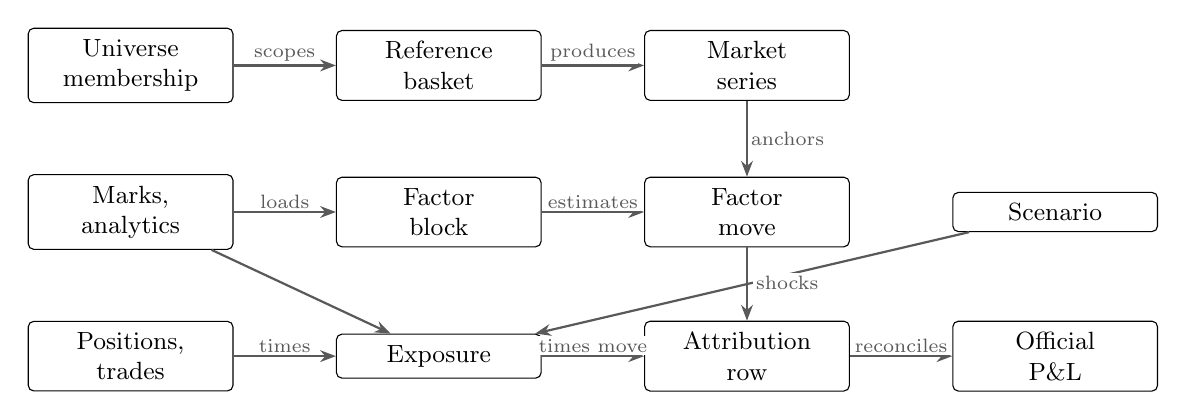
\begin{tikzpicture}[node distance=9mm and 13mm,every edge quotes/.style={}]
\node[box] (univ) {Universe\\membership};
\node[box,right=of univ] (basket) {Reference\\basket};
\node[box,right=of basket] (series) {Market\\series};
\node[box,below=of univ] (marks) {Marks,\\analytics};
\node[box,right=of marks] (fblock) {Factor\\block};
\node[box,right=of fblock] (fmove) {Factor\\move};
\node[box,below=of marks] (pos) {Positions,\\trades};
\node[box,right=of pos] (expo) {Exposure};
\node[box,right=of expo] (attr) {Attribution\\row};
\node[box,right=of attr] (pnl) {Official\\P\&L};
\node[box,right=of fmove] (scen) {Scenario};
\draw[dep] (univ)--node[above,font=\scriptsize,fill=white,inner sep=1pt]{scopes}(basket);
\draw[dep] (basket)--node[above,font=\scriptsize,fill=white,inner sep=1pt]{produces}(series);
\draw[dep] (marks)--node[above,font=\scriptsize,fill=white,inner sep=1pt]{loads}(fblock);
\draw[dep] (fblock)--node[above,font=\scriptsize,fill=white,inner sep=1pt]{estimates}(fmove);
\draw[dep] (series)--node[right,font=\scriptsize,fill=white,inner sep=1pt]{anchors}(fmove);
\draw[dep] (pos)--node[above,font=\scriptsize,fill=white,inner sep=1pt]{times}(expo);
\draw[dep] (marks)--(expo);
\draw[dep] (expo)--node[above,font=\scriptsize,fill=white,inner sep=1pt]{times move}(attr);
\draw[dep] (fmove)--(attr);
\draw[dep] (attr)--node[above,font=\scriptsize,fill=white,inner sep=1pt]{reconciles}(pnl);
\draw[dep] (scen)--node[right,font=\scriptsize,fill=white,inner sep=1pt]{shocks}(expo);
\end{tikzpicture}
\end{center}

\subsection{Rate of change}
\begin{itemize}
\item \textbf{Stable:} the canonical schema, units and signs, reading statuses, the \code{Source} port.
\item \textbf{Moderate:} basket, factor and scenario definitions; the attribution model version; calculation code.
\item \textbf{Volatile:} the data adapters (they differ by machine), the data itself, the screens.
\end{itemize}
The boundaries follow from this. The volatile adapters sit at the edge. The stable schema sits at the centre. Definitions are files, so they change without code changes.

\subsection{Modules}
\begin{center}\footnotesize
\begin{tabularx}{\linewidth}{@{}l>{\raggedright}p{3.2cm}>{\raggedright}p{3.1cm}>{\raggedright}p{3.1cm}X@{}}\toprule
Module & Responsibility & Knows about & Does not know about & Changes when \\\midrule
\code{crw.domain} & The shared vocabulary & Schemas, units, signs, statuses, run context, definition types & Any data source, any calculation & The brief's contract changes \\
\code{crw.data} & Reading data safely & The port, the view, adapters, the checker & What calculations do with data & A machine or vendor changes \\
\code{crw.book} & Positions and accounting & Roll-forward, reconciliation, ETF look-through & Factors, baskets, storage & Accounting rules change \\
\code{crw.exposure} & Sensitivities & CS01, dollar DTS, key rates, aggregation & Where marks come from & Sensitivity conventions change \\
\code{crw.baskets} & Market measures & Eligibility, weights, caps, pair normalisation, gaps and ratios & The book & A basket definition changes \\
\code{crw.factors} & Factor moves & Factor blocks, loadings, the estimator & Positions, P\&L & The attribution model changes \\
\code{crw.attribution} & Explaining P\&L & Carry, rates, factor, ETF layers, residual, bridge & Storage, screens & Attribution rules change \\
\code{crw.results} & Storing outputs & Result schemas, the result store & How results were computed & An output table is added \\
\code{crw.runs} & Running a day & Order of steps, manifest, archive, wiring & Calculation internals & The daily process changes \\
\code{crw.app} & Screens (later) & Result tables & Calculations and sources & The UI changes \\\bottomrule
\end{tabularx}
\end{center}
Later layers add \code{crw.diagnostics} (Layer 4) and \code{crw.risk} (Layer 5). The review below says not to create them yet.

\subsection{Abstraction decisions}
\begin{itemize}
\item \textbf{Protocol} for \code{Source}: there are three implementations from day one (synthetic, tables, archive), and the work adapter is the fourth.
\item \textbf{Protocol} for \code{FactorBlock}: common, quality, sector and curve blocks vary in how they build loadings.
\item \textbf{Protocol} for \code{ResultStore}: parquet store and in-memory store for tests.
\item \textbf{Class} for \code{View}: it holds the source, the as-of time and the read recorder.
\item \textbf{Functions} for every calculation: CS01, DTS, basket returns, attribution. They are stateless.
\item \textbf{Dataclasses} (frozen) for \code{RunContext}, \code{Window}, definitions and the manifest.
\item \textbf{Config} as YAML files loaded into frozen dataclasses (see Section~\ref{sec:config}).
\end{itemize}

\subsection{Dependency direction}
All arrows point to \code{crw.domain}. Calculation packages import only \code{crw.domain} and each other in one direction: \code{book} $\to$ \code{exposure} $\to$ \code{factors} $\to$ \code{attribution}, and \code{baskets} $\to$ \code{factors}. Only \code{crw.runs} imports \code{crw.data} and \code{crw.results}. Nothing imports \code{crw.runs} except the CLI. The graph is a DAG.

%======================================================================
\section{Design}
%======================================================================

\subsection{Objective and core abstraction}
\textbf{Objective.} Turn one day's canonical inputs into exposures, market measures, an additive P\&L explanation and scenario losses, each with a status and a version, reproducible from its archive.

\textbf{Core abstraction: the canonical table read as of a time.} Everything else orbits it. A calculation never asks ``where is the data''. It receives ``these rows, known by this time, in these units''. If the requirements change, new kinds join the schema. The abstraction holds.

\subsection{Components}
\begin{center}\small
\begin{tabularx}{\linewidth}{@{}lXll@{}}\toprule
Component & One responsibility & Uses & Used by \\\midrule
Domain core & Defines the canonical vocabulary & nothing & all \\
Data access & Serves validated point-in-time tables & domain & runs \\
Measurement engines & Compute exposures, measures, attribution & domain & runs \\
Results store & Persists outputs with status and version & domain & runs, app \\
Run orchestration & Wires one day's steps and archives them & data, engines, results & CLI \\
Presentation (later) & Shows results & results & user \\\bottomrule
\end{tabularx}
\end{center}

\subsection{Dependency graph}
\begin{center}
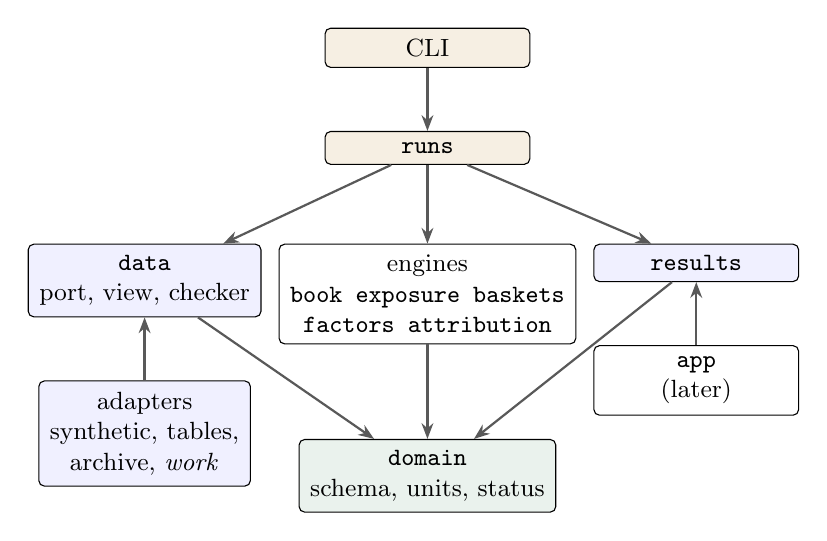
\begin{tikzpicture}[node distance=8mm and 10mm]
\node[orch] (cli) {CLI};
\node[orch,below=of cli] (runs) {\code{runs}};
\node[infra,below left=10mm and 8mm of runs] (data) {\code{data}\\port, view, checker};
\node[box,below=10mm of runs,minimum width=3.4cm] (eng) {engines\\\code{book exposure baskets}\\\code{factors attribution}};
\node[infra,below right=10mm and 8mm of runs] (res) {\code{results}};
\node[dom,below=12mm of eng] (dom) {\code{domain}\\schema, units, status};
\node[infra,below=of data] (ad) {adapters\\synthetic, tables,\\archive, \emph{work}};
\node[box,below=of res] (app) {\code{app}\\(later)};
\draw[dep] (cli)--(runs);
\draw[dep] (runs)--(data); \draw[dep] (runs)--(eng); \draw[dep] (runs)--(res);
\draw[dep] (data)--(dom); \draw[dep] (eng)--(dom); \draw[dep] (res)--(dom);
\draw[dep] (ad)--(data); \draw[dep] (app)--(res);
\end{tikzpicture}
\end{center}
Engines never import \code{data} or \code{results}. Adapters depend on the port; the port does not know any adapter. The CLI picks the adapter through \code{CRW\_SOURCE}.

\subsection{Data flow for one day}
\begin{enumerate}
\item \textbf{Open.} \code{runs} builds a \code{RunContext}: book, currency, interval $[t_0,t_1]$, the opening position time, the current position time, the attribution version, the as-of time.
\item \textbf{Read.} The view reads each kind for the window. \emph{Format:} pandas DataFrame with the canonical columns. \emph{Failure:} schema violation raises; a missing kind raises \code{DataUnavailable}; a row known after the as-of time is dropped, and a direct request for it raises \code{LookAheadError}.
\item \textbf{Book.} Roll positions forward from trades and events. Reconcile to official P\&L. Build ETF look-through holdings. \emph{Output:} positions with a \code{position\_basis} column (actual or synthetic).
\item \textbf{Exposure.} CS01, $K_i = V_i D^s_i s_i$, key rates, per security, then cash long, cash short, ETF and net.
\item \textbf{Measures.} Basket weights at $t_0$, basket levels and moves at $t_1$, gaps and log ratios.
\item \textbf{Factors.} Loadings at $t_0$ from each block. Common move $m_t$ from the anchor basket. Remaining factor moves from the estimator.
\item \textbf{Attribution.} Per security first: carry, rates, each factor, ETF layers, residual. Then aggregate. Then the bridge: actual P\&L $=$ components $+$ reconciliation difference.
\item \textbf{Write.} Each result table goes to the store with \code{run\_id}, \code{model\_version} and a status per row. The manifest lists inputs, definition hashes and exceptions. The recorded input frames go to the archive.
\end{enumerate}
\textbf{Failure policy.} A step that fails marks its outputs \code{unavailable} and the run \code{incomplete}. It never writes zeros. A rerun with late data writes a new \code{run\_id} that names the run it revises.

\subsection{Mathematical contract}
Spreads are decimal in all calculations. Display converts to bp.
\[
CS01_i = V_i D^s_i 10^{-4},\qquad K_i = V_i D^s_i s_{i,0},\qquad z_i = \frac{\Delta s_i}{s_{i,0}},\qquad \Delta P^{credit}_i \approx -K_i z_i .
\]
\textbf{Factor model (initial).} With $\beta=1$ and the common move $m_t$ fixed by the anchor basket:
\[
z_{i,t} - m_t = q_{i,t-1}^{\top}Q_t + a_{i,t-1}^{\top}S_t + c_{i,t-1}^{\top}C_t + u_{i,t}.
\]
Weighted least squares across the reference universe each day. Quality uses B as the reference group, so $Q = (Q_{BB/B}, Q_{CCC/B})$ are two contrasts. Sector effects sum to zero under the universe's DTS weights, so they cannot carry the common move. Factor exposure and P\&L are
\[
E_{k,t-1} = \sum_i K_{i,t-1} x_{ik,t-1}, \qquad P\&L_{k,t} \approx -E_{k,t-1} f_{k,t}.
\]
\textbf{Where it breaks.}
\begin{itemize}
\item \textbf{Empty cell.} A sector with no names that day has no column. Its factor gets status \code{unavailable}, not zero.
\item \textbf{Singular design.} The sum-to-zero constraint plus the reference group removes the redundancy. The estimator checks the rank and refuses if it is short.
\item \textbf{Distressed bonds.} Above a definition-set spread or below a price threshold, a bond leaves the proportional model. Its P\&L goes to an explicit ``price-mode exception'' line.
\item \textbf{Overfitting.} None is estimated across days in the first model. The reserved validation dates from the brief's P0 task stay out of every tuning step.
\end{itemize}

\subsection{Key interfaces}
\begin{lstlisting}
from __future__ import annotations

from dataclasses import dataclass
from datetime import datetime
from enum import Enum
from typing import Protocol, runtime_checkable

import pandas as pd


class Kind(str, Enum):
    """The canonical tables (brief Section 9). Schemas live in crw.domain.schema."""
    SECURITIES = "securities"
    UNIVERSE = "universe"
    TAXONOMY = "taxonomy"
    POSITIONS = "positions"
    TRADES = "trades"
    OFFICIAL_PNL = "official_pnl"
    MARKS = "marks"
    ANALYTICS = "analytics"
    CURVES = "curves"
    ETF_MARKET = "etf_market"
    ETF_HOLDINGS = "etf_holdings"


@dataclass(frozen=True)
class Window:
    """Rows whose effective_at lies in [start, end]."""
    start: datetime
    end: datetime


@runtime_checkable
class Source(Protocol):
    """One machine's data. Returns every revision of canonical rows, each with
    effective_at and available_at. Point-in-time filtering is the View's job."""

    def kinds(self) -> frozenset[Kind]: ...
    def read(self, kind: Kind, window: Window) -> pd.DataFrame: ...


@runtime_checkable
class FactorBlock(Protocol):
    """One family of attribution factors (common, quality, sector, curve)."""

    block_id: str

    def loadings(self, cross_section: pd.DataFrame) -> pd.DataFrame:
        """Index security_id, one column per factor_id, from data known at t0."""
        ...


@runtime_checkable
class ResultStore(Protocol):
    """Where a run's output tables go. Rows carry run_id, model_version, status."""

    def write(self, table: str, frame: pd.DataFrame, run_id: str) -> None: ...
    def read(self, table: str, run_id: str) -> pd.DataFrame: ...
\end{lstlisting}
The view is a concrete class: \code{View(source, as\_of, recorder).get(kind, window)}. It validates the schema, drops rows with \code{available\_at} after \code{as\_of}, keeps the latest revision per key, and records the frame it returns.

\subsection{Configuration}\label{sec:config}
\textbf{Approach: Dataclasses.} YAML files load into frozen dataclasses with explicit validation. This overrides the design skill's Pydantic default. Reasons: your HY Analyst repo uses the same approach, and the work machine may restrict packages. Each extra runtime dependency is one more approval at work.
\begin{itemize}
\item \code{definitions/baskets/*.yaml}, \code{definitions/factors/*.yaml}, \code{definitions/scenarios/*.yaml}: each has \code{id} and \code{version}. The manifest stores a content hash.
\item \code{config/run.yaml}: book, currency, universe id, data root, as-of rule.
\item Environment: \code{CRW\_SOURCE} (adapter), \code{CRW\_DATA\_ROOT} (tables and archive), \code{CRW\_RESULTS\_ROOT}.
\end{itemize}

\subsection{Errors}
\begin{itemize}
\item \textbf{Data layer:} raise on schema violation, \code{DataUnavailable}, \code{LookAheadError}. Adapters may retry network reads. The view never fills gaps.
\item \textbf{Engines:} a missing input for one security gives that security's rows status \code{unavailable}. They do not stop the day.
\item \textbf{Runs:} catch per step, mark the run \code{incomplete}, write the exception to the manifest, exit non-zero.
\end{itemize}

\subsection{Testing}
\begin{itemize}
\item \textbf{Unit:} every formula in Section 8 of the brief, including the 10.1 example (\$0 and $-\$10{,}000$) and the ETF identity.
\item \textbf{Acceptance:} one test per row of the brief's Section 10 table, run on the synthetic source.
\item \textbf{Recovery:} the synthetic market draws known factor moves; the estimator must recover them within a tolerance on a held-out seed.
\item \textbf{Contract:} the checker passes on the synthetic and tables sources; a deliberately broken source (bp spreads, future rows, positive short) must fail each check.
\item \textbf{Boundary:} an import test fails if any engine imports \code{crw.data}, \code{crw.results} or \code{crw.runs}.
\item \textbf{Replay:} a run, then a replay from its archive, gives identical results.
\end{itemize}

\subsection{File structure}
\begin{lstlisting}[language={},basicstyle=\ttfamily\footnotesize]
risk-workbench/
|-- pyproject.toml
|-- config/run.yaml
|-- definitions/            baskets/, factors/, scenarios/  (versioned YAML)
|-- docs/design/            this document; data_contract.md; work_machine.md
|-- src/crw/
|   |-- domain/             schema.py  units.py  status.py  context.py
|   |                       definitions.py  errors.py
|   |-- data/               source.py  view.py  factory.py  contract.py
|   |   `-- adapters/       synthetic.py  tables.py  archive.py  composite.py
|   |-- book/               positions.py  reconcile.py  lookthrough.py
|   |-- exposure/           sensitivities.py  aggregate.py
|   |-- baskets/            weights.py  measures.py
|   |-- factors/            blocks.py  estimate.py
|   |-- attribution/        credit.py  carry_rates.py  etf.py  bridge.py
|   |-- results/            store.py  tables.py
|   |-- runs/               daily.py  manifest.py
|   `-- cli.py
`-- tests/                  unit/  acceptance/  contract/  test_boundaries.py
\end{lstlisting}

\subsection{Build plan}
Each step ends with something usable, as the brief requires. Times are agent working time, assuming no surprises.
\begin{center}\small
\begin{tabularx}{\linewidth}{@{}lXXl@{}}\toprule
Step & Build & Usable output & Time \\\midrule
M0 & Domain schema, port, view, factory, checker, synthetic and tables sources, result store, manifest & \code{crw check-source} passes on synthetic data & 1 day \\
M1 (Layer 0) & Roll-forward, reconciliation, CS01, dollar DTS, key rates, cash/ETF/net & Position and issuer report with coverage & 1--2 days \\
M2 (Layer 1) & Market diary, carry and rates, common credit, ETF layers, residual & ``Did the hedge offset the common move?'' & 2 days \\
M3 (Layer 2) & Basket engine, B/BB, CCC/B, largest sector pairs & Market monitor with drill-down & 2--3 days \\
M4 (Layer 3) & Factor blocks, estimator, bridge, versioning & Additive P\&L bridge & 3 days \\
Later & Layers 4--6, screens, work adapter & & \\\bottomrule
\end{tabularx}
\end{center}
M0 to M4 are file-disjoint enough for \code{orchestrate} after M0 lands. M0 itself should be one agent, because every later step depends on the schema.

\subsection{Risks and what we deliberately skip}
\begin{itemize}
\item \textbf{Risk:} the canonical schema is wrong in a way only the work data reveals. \emph{Mitigation:} write \code{docs/design/data\_contract.md} early, and take it to work before M2.
\item \textbf{Risk:} the local fallback pricer (spread duration from yield and maturity) is crude. It is only for synthetic and TRACE data. At work, vendor analytics replace it.
\item \textbf{Skipped:} screens, intraday, multi-currency, covariance, hedge comparison. The brief puts them later.
\item \textbf{Skipped:} a local real-data adapter for TRACE. Its duplicate rows make it unfit for attribution tests.
\end{itemize}

%======================================================================
\section{Architecture review of this design}\label{sec:review}
%======================================================================
No code exists yet, so this review scores the proposed structure, not files. It uses the seven dimensions of the review-architecture skill.

\begin{center}\small
\begin{tabularx}{\linewidth}{@{}llX@{}}\toprule
Dimension & Score & Key finding \\\midrule
Boundary quality & \color{good}Strong & Modules follow rate of change; \code{attribution} needs watching \\
Dependency direction & \color{good}Strong & All arrows point to \code{domain}; enforced by a test \\
Abstraction fitness & \color{warn}Adequate & Generic \code{read(kind)} trades type safety for portability \\
DRY and knowledge & \color{warn}Adequate & Column names and units are shared strings: one home needed \\
Extensibility & \color{good}Strong & New source: 1 new file. New factor: 1 file plus 1 YAML \\
Testability & \color{good}Strong & Engines are pure; runs needs 3 fakes \\
Parallelisation & \color{warn}Adequate & Days are independent, but the read recorder is shared state \\\bottomrule
\end{tabularx}
\end{center}
\textbf{Overall: \color{good}sound\color{black}. Fix three things before code.}

\subsection*{Fix before code}
\begin{description}
\item[AR-PAR-001 (Adequate).] \code{View} holds a recorder that collects every frame read. If days run in parallel workers, one shared recorder is mutable shared state. \emph{Direction:} one view and one recorder per day per worker. The run merges archives after the workers finish.
\item[AR-DRY-001 (Adequate).] Engines, the checker and the result store all use column names and units. As strings, they drift. \emph{Direction:} \code{crw.domain.schema} owns every column name, dtype and unit. Nothing else writes a literal column name.
\item[AR-ABS-001 (Adequate).] \code{read(kind, window)} returns an untyped frame. A wrong frame fails late. \emph{Direction:} the view validates against the kind's schema on every read, so the failure happens at the boundary. Accept the trade-off; do not add per-kind methods.
\end{description}

\subsection*{Watch during build}
\begin{description}
\item[AR-BND-001 (Adequate).] \code{attribution} will gather carry, rates, factors, ETF layers, residuals and the bridge. \emph{Direction:} keep the bridge as the only module that sees all components; split further if a file passes 300 lines.
\item[AR-BND-002 (Adequate).] Basket rules name sectors. Sector codes differ by machine. \emph{Direction:} definitions use canonical sector codes only; the \code{taxonomy} kind maps source codes to them.
\item[AR-EXT-001 (Weak, inherent).] A new canonical kind touches the schema, the checker, the tables adapter and the synthetic adapter: four files. \emph{Direction:} accept it, because kinds change rarely. Generate the schema-driven parts in the tables adapter from the schema, so it needs no edit.
\item[AR-ABS-002 (Adequate).] Do not create \code{diagnostics} or \code{risk} packages before Layers 4 and 5. Empty packages invite misplaced code.
\end{description}

\subsection*{What to keep}
\begin{itemize}
\item Snapshot on read: it turns reproducibility from a process into a property.
\item Status on every result row: it makes ``missing is not zero'' structural, not a UI convention.
\item The same port shape as \code{hy.data}: one mental model across both repos.
\end{itemize}

%======================================================================
\section{Agreed in review, 25 October 2026}\label{sec:agreed}
%======================================================================
These points came out of the discussion of this document. They \textbf{override} earlier sections where the two differ.

\subsection{The production machine has}
\begin{itemize}
\item \textbf{Intraday bond prices from MarketAxess CP+}, at regular intervals, with a timestamp per bond.
\item \textbf{FINCAD} for analytics (OAS, spread duration, key rates), callable directly from Python.
\end{itemize}

\subsection{Changes to the design}
\begin{enumerate}
\item \textbf{The data-layer cut stands.} One canonical schema, one \code{Source.read(kind, window)} port, a point-in-time view, snapshot on read.
\item \textbf{Three run modes, not one daily run.}
  \begin{itemize}
  \item \emph{Start of day:} opening positions, sensitivities, factor loadings and basket weights, computed once.
  \item \emph{Refresh:} every few minutes, latest prices $\to$ factor moves $\to$ P\&L. Only this part reruns.
  \item \emph{End of day:} the last refresh plus the official P\&L reconciliation.
  \end{itemize}
  \code{RunContext.as\_of} is a datetime, not a date. Semi-live is built after M2 (about 2--3 days). The start-of-day/refresh split is built from M0 (about 1 extra day).
\item \textbf{Prices are a stream.} The view takes, per bond, the latest price at or before the refresh time. A price may be used only once it has \emph{arrived} (\code{available\_at}). Its age is measured from \emph{its own} timestamp (\code{observed\_at}).
\item \textbf{Stale is per bond, and not only by age.} CP+ publishes on a schedule, so a fresh timestamp can carry a model-carried price. A bond is flagged stale when (a) its price age exceeds a limit set in a settings file (start: one limit, for example 30 minutes), or (b) its price has not changed for a set number of intervals, or (c) a CP+ quality field, if the feed carries one, says so. A stale bond's P\&L goes on a stale line, never to zero.
\item \textbf{Intraday moves use fresh bonds only}, and show their coverage (for example ``1,240 of 1,900 repriced''). Liquid bonds reprice more often, so coverage must sit next to every intraday move.
\item \textbf{Price moves become spread moves by a labelled first-order rule} until FINCAD repricing is fast enough: price change since the open, minus the Treasury move times the opening rate sensitivity, divided by the opening spread duration. CP+ benchmark spreads are not OAS and are not mixed with FINCAD OAS.
\item \textbf{ETF prices are taken at the refresh time}, and a gap between bond and ETF timestamps is flagged.
\item \textbf{Intraday positions} are opening positions plus trades so far. P\&L is split at each trade time.
\item \textbf{Price source: CP+ for both refresh and close, set in settings.} Each price row carries a \code{source} column. Settings name the refresh source and the close source. A ``price source change'' P\&L line switches on only when they differ. A gap to the desk's official P\&L shows on the reconciliation line.
\item \textbf{A pricer port joins the design.}
\begin{lstlisting}
@runtime_checkable
class Pricer(Protocol):
    """Analytics for bonds at given prices. Spreads are decimal; durations positive."""

    def analytics(self, terms: pd.DataFrame, prices: pd.DataFrame,
                  curve: pd.DataFrame) -> pd.DataFrame: ...
\end{lstlisting}
  \begin{itemize}
  \item Chosen by \code{CRW\_PRICER=module:factory}, the same pattern as \code{CRW\_SOURCE}.
  \item Here: a simple local pricer for plain fixed-coupon bonds; callables get status \code{estimated}.
  \item At work: a FINCAD adapter.
  \item Start of day: FINCAD output is stored and archived as the \code{analytics} table.
  \item Scenarios and callables use full repricing through the port. Intraday full repricing replaces the first-order rule once its speed is measured at work.
  \item A \textbf{pricer check} prices a set of plain bonds with known answers. It checks that OAS is decimal, spread duration is positive, and key rates sum to about the duration.
  \item Pricing runs bond by bond. It is sequential by default, because the FINCAD licence may not allow parallel calls. A setting turns parallel on.
  \end{itemize}
\end{enumerate}

\subsection{Still open}
\begin{enumerate}
\item \textbf{Positions and trades:} which system or systems at work. If several, a \code{CompositeSource} routes each kind.
\item \textbf{Package name:} \code{crw} proposed, not confirmed.
\item \textbf{Dataclasses or Pydantic:} dataclasses proposed, not confirmed.
\item \textbf{Section 13 defaults for M0--M2:} proposed USD only, ICE-style HY universe rules, B as the quality reference group. Not confirmed.
\item \textbf{CP+ fields:} whether the feed carries a quality or confidence field (used by the stale rule).
\item \textbf{FINCAD speed} for about 2,000 bonds, which decides intraday full repricing.
\end{enumerate}

\subsection{First steps on the production machine}
\begin{enumerate}
\item Answer the open items above, starting with positions and trades.
\item Build M0 there, including the start-of-day/refresh split and the pricer port.
\item Write the CP+ source adapter and the FINCAD pricer adapter.
\item Run the data check and the pricer check. Fix every failed required row before M1.
\end{enumerate}

\end{document}
